
\documentclass[12pt,oneside,a4paper]{article}

\usepackage{graphicx}
\usepackage{listings}	
\usepackage{hyperref}
\usepackage{url} 

\usepackage[margin=10pt,font=footnotesize,labelfont=bf]{caption}

\parindent 0pt
\parskip 10pt

\begin{document}






\title{
Simulation of Gaussian Random Fields using NVIDIAs CUDA: the \textbf{gpusim} package \\
Version 0.01
\vspace{1in}}

\author{
Marius Appel\footnote{Institute for Geoinformatics, University of Muenster, Germany.} \\
\ttfamily{marius.appel@uni-muenster.de}
\vspace*{\fill}}

\maketitle

\newpage


\tableofcontents

\newpage

\section{Introduction}
With publication of NVIDIAs Compute Unified Device Architecture (CUDA), a new approach for general purpose programming of graphics processing units (GPU) was available. Due to the highly parallel architecture of GPUs, researchers from different domains found out that GPUs have the power to accelerate parallel computation tasks in many applications strongly. 
Our gpusim package takes advantages of the highly parallel architecture of GPUs too. It provides methods for simulation of gaussian random fields. For unconditional simulation, our implementation works in the spectral domain in order to benefit from NVIDIAs CUFFT library, an efficient implementation of FFTs on GPUs. Furthermore, our package uses the CURAND library for fast random number generation and the CUBLAS library for an efficient matrix vector product. The conditional simulation takes advantage of an efficient implementation of kriging prediction on GPUs based on \cite{srinivasan:kriging}.


\section{Installation}
\subsection{System Requirements}

Operating System: Microsoft Windows 7 and Linux systems are currently supported.
 
Because gpusim uses NVIDIAs CUDA for GPU computing, you need suitable hardware equipment and recent graphics drivers. 
Furthermore, you need NVIDIAs GPU Computing Toolkit including cufft, cublas and curand libraries. In order to achieve maximum performance, you should always use the latest version of your drivers and the toolkit.
The package needs R version 2.12.1 or higher and depends on the packages gstat \cite{pkg:gstat} and \cite{pkg:fields}. 



\subsection{Installation on Linux platforms}
On Linux platforms you have to compile the package from source. Since the source code has to be linked to the CUDA libraries, you maybe will have to change the path of the CUDA installation in \verb|src/Makefile| if you installed CUDA to a user-defined path. By default, 64 bit libraries are used. If this doesn't fit to your environment, change the \verb|CUDA_LIB_PATH| entry in the Makefile. 
For compilation and installation just type \verb|R CMD INSTALL gpugeo| in your terminal. 




\subsection{Installation on Windows platforms}
For Microsoft Windows platforms, there is a binary release available for download. After downloading the .zip file, you can simply install the package in the RGui by selecting \verb|packages -> install packages from local zip files| in the menu. 
Note that there are different versions for 32 and 64 Bit systems. However, if you want to compile it on your own, you will need Rtools and a VisualC++ 2008 / 2010 installation. For details about compilation problems in Windows, just contact us.








\section{Getting Started}
At first,  start R and load the package by typing:
\verb|> library(gpugeo)|
During package loading, the first CUDA capable GPU on your system is detected and initialized automatically. An error will occur, if no qualified GPU can be found. In this case, you should check your hardware configuration and install recent graphics drivers and the CUDA toolkit including NVIDIAs cufft, cublas and curand libraries.
 

\subsection{Unconditional Simulation}
For performing an unconditional simulation, the first step is to define the grid. The \emph{gpuSim()} function takes a GridTopology or a SpatialPixelsDataFrame object as an argument defining the grid. Usually you can define a GridTopology object based on six parameters: two coordinates of the upper left corner, two numbers defining the width / height of a cell and two integers defining the number of rows / columns. The following code shows an example how to build a grid:

\begin{verbatim}
# build grid
xmin = 0
xmax = 5
ymin = 0
ymax = 5
nx = 100
ny = 100
dx = (xmax-xmin)/nx
dy = (ymax-ymin)/ny
grid = GridTopology(c(xmin,ymin), c(dx,dy), c(nx,ny))
\end{verbatim}


The second step is to define a covariance function. For meaningful results you should always fit a function to real data but this is not what gpusim is made for. You can use the gstat package \cite{pkg:gstat} to fit a variogram to samples.
Currently, three different covariance functions are implemented and listed below. Each function is defined by a sill, a range and a nugget parameter, denoted as $s$, $r$ and $n$ respectively. All three models are in accord with gstat definitions.


Exponential covariance function:
\begin{displaymath}
  C_{exp}(h) = 
   \left\{ 
    \begin{array}{cc}
                 s \cdot e^{\frac{-h}{r}} & if \quad h > 0  \\
                 s + n & if \quad h = 0  
    \end{array} 
   \right.
\end{displaymath}
 
 
Gaussian covariance function:
\begin{displaymath}
  C_{gau}(h) = 
   \left\{ 
    \begin{array}{cc}
                 s \cdot e^{-\left(\frac{h}{r}\right)^{2}} & if \quad h > 0  \\
                 s + n & if \quad h = 0  
    \end{array} 
   \right.
\end{displaymath}
 
 
Spherical covariance function:
\begin{displaymath}
  C_{sph}(h) = 
   \left\{ 
    \begin{array}{cc}
                 s \cdot\left( 1 - \left( \frac{3h}{2r} - \frac{h^3}{2r^3} \right) \right) & if \quad 0 < h \leq r  \\           
                 s + n & if \quad h = 0 \\
                 0 & if \quad h < r
                 
    \end{array} 
   \right.
\end{displaymath}
 
 
 
In the \emph{gpuSim()} function, a model is specified by four arguments:
\begin{itemize}
	\item A character identifier defining the covariance model, currently `Exp', `Gau' or `Sph'
	\item Three numerical values for sill, range, nugget parameter
\end{itemize}

Users can choose the output type of the resulting grids. The boolean argument \emph{as.sp} specifies, whether the result type is conform with the sp package as a SpatialPixelsDataFrame object or the result is a simple three-dimensional array, with the third index denoting the realization, the second index denoting the row and the first index denoting the column in a grid.
In order to achieve maximum performance, use as.sp = FALSE.

The following code shows a simple example for executing an unconditional simulation:
\begin{verbatim}
# build grid
xmin = 0
xmax = 5
ymin = 0
ymax = 5
nx = 100
ny = 100
dx = (xmax-xmin)/nx
dy = (ymax-ymin)/ny
grid = GridTopology(c(xmin,ymin), c(dx,dy), c(nx,ny))

# covariance arguments
model = "Gau"
range = 0.5
sill = 3
nugget = 0

k = 5  ## number of realizations

# unconditional simulation (result as array)
simGPU = gpuSim(grid, model, sill, range, nugget, k)
image.plot(simGPU[,,5]) ## plot 5-th realization

# unconditional simulation with sp interoperability
simGPUsp = gpuSim(grid, model, sill, range, nugget, k, as.sp = TRUE)
spplot(simGPUsp) # plot all realizations using sp
\end{verbatim}



\subsection{Conditioning}
Once you have a set of unconditional realizations and want to condition them by sample data, you can pass samples to the \emph{gpuSim()} function as a SpatialPointsDataFrame object from the sp package with exactly one data attribute. If you are not familiar with sp classes, the following examples will show how to make it:

\begin{verbatim}
# generate random samples...
n = 100 ## number of samples
sample_x = runif(n,min=0,max=5) # sample x coords
sample_y = runif(n,min=0,max=5) # sample y coords
sample_z = rnorm(n,20,4) ## sample values, e.g temperature
samples = data.frame(x=sample_x, y=sample_y)
coordinates(samples)=c("x","y") # designate x and y column as coordinates
samples = SpatialPointsDataFrame(samples,as.data.frame(sample_z))
\end{verbatim}

Calling the following code after generating unconditional realizations as seen above, fulfills the conditioning step.
\begin{verbatim}
# conditioning using unconditional realizations computed before
simGPUcond1 = gpuSim(grid,model,sill,range,nugget,samples=samples,
                     uncond=simGPU)
image.plot(simGPUcond1[,,5])
\end{verbatim}



\subsection{Conditional Simulation}
Instead of executing the generation of unconditional realizations and the following conditioning separately, you can do this with only one call of \emph{gpuSim()} and a better performance.
Just build the grid, the covariance function and the samples as written above and run \emph{gpuSim()} in the following way:

\begin{verbatim}
# conditional simulation without sp interoperability
simGPUcond = gpuSim(grid, model, sill, range, nugget, k, samples)
image.plot(simGPUcond[,,5]) ## plot 5-th realization

# conditional simulation with sp interoperability
simGPUcondsp = gpuSim(grid, model, sill, range, nugget, k, samples,
                      as.sp = TRUE)
spplot(simGPUcondsp) # plot all realizations using sp
\end{verbatim}




\section{Performance Checking}
In order to get an overview of the performance, there is a \emph{gpuSimEval()} function, which takes the same arguments as the \emph{gpuSim()} function, but returns only needed computation times for different required steps of the simulation. For instance a unconditional simulation in \emph{gpuSimEval()} returns the time needed for GPU preprocessing, which only depends on the grid size, the time needed for generating all realizations which additionally depends on the number of realizations and the time that is needed for remaining time needed for CPU execution (e.g. creating an sp object). More details can be found in the documentation of \emph{gpuSimEval()}.


\section{Internal Grid Representation}
Internally, all grids are stored in row-major order. For interoperability with sp, spatial coordinates are stored in a usual cartesian system (no image coordinates) - with origin at the lower left corner. An array result of a simulation is always returned three dimensionally. Accessing a specific pixel of a realization is done by \verb|grid[col,row,realization]|, where col and row are the image coordinates (pixels) with (0,0) at the upper left corner. These details are illustrated in the example grid below.

\begin{center}
	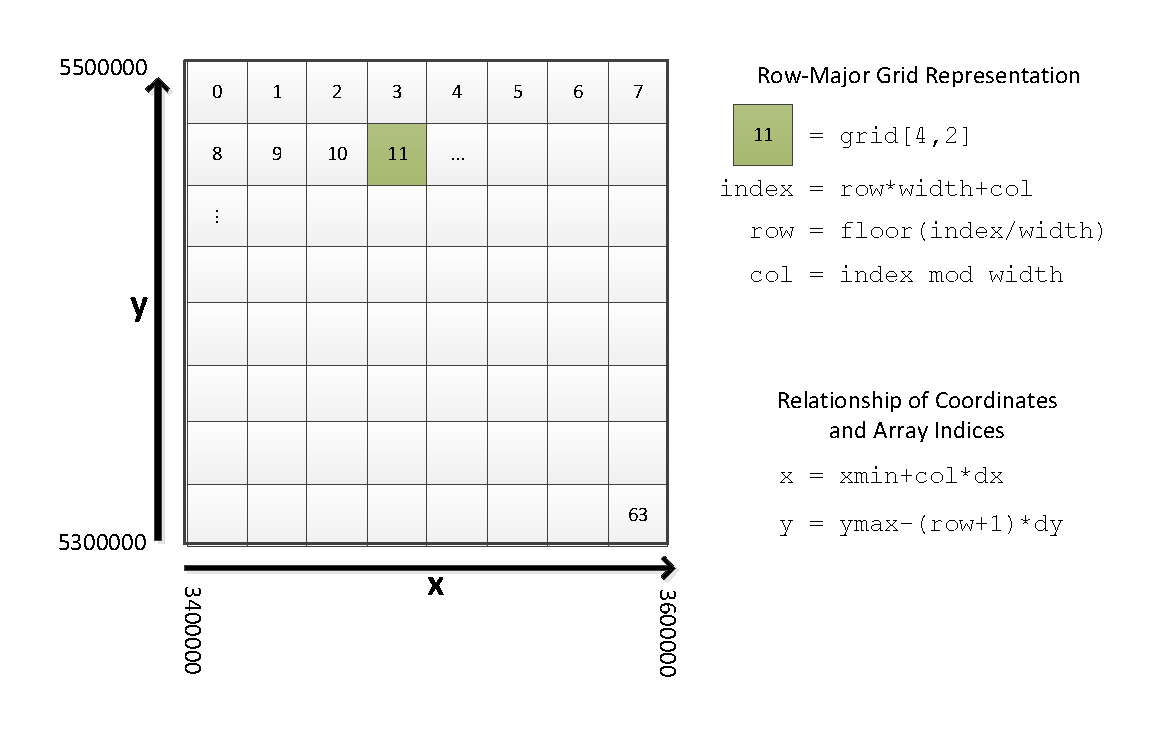
\includegraphics[scale=0.65]{grid.pdf}
\end{center}



\bibliography{gpusim}
 \bibliographystyle{plain}
  
  
\end{document}





